\section{Meta-cognition}
    \cite{metcalfe-1994-metacognition-knowing-about-knowing} defines metacognition is an awareness of one's thought processes and an understanding of the patterns behind them.
    \begin{frame}{Mind > Cognition > Processes}
        \begin{figure}[H]
            \centering
            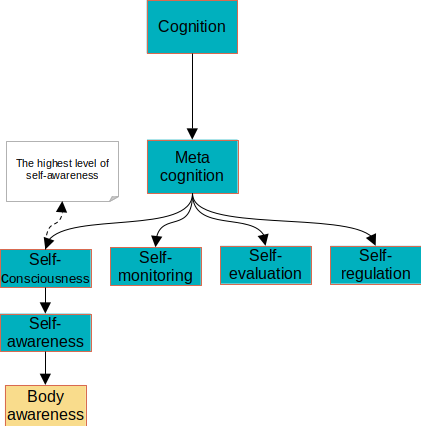
\includegraphics[width=0.9\textwidth]{anatomy/mind/cognition/meta_cognition.png}
        \end{figure}
    \end{frame}
    Meta-cognition is considering own cognition
    \begin{itemize}
        \item Having the capability to continuously monitor perceptions and improve them
    \end{itemize}